\documentclass{standalone}
\usepackage{tikz}
\begin{document}
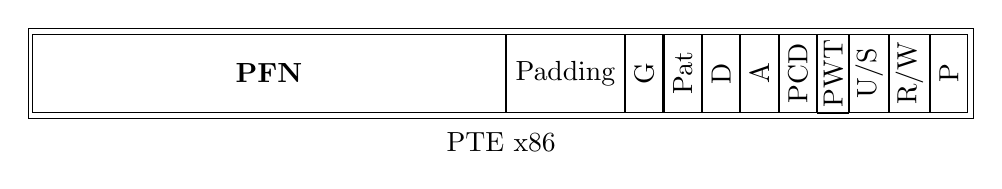
\begin{tikzpicture}
    \draw
    
    (-0.05,-1)node[draw, rectangle, minimum height=1.15cm, minimum width=12cm, anchor=180, label={[label distance=-1.7cm]:PTE x86}]{}
    (0,-1)node[draw, rectangle, minimum width=6cm, minimum height=1cm, fill=white, align=center, anchor=180](e0){\textbf{PFN}}
    (e0.0)node[draw, rectangle, minimum width=1.5cm, minimum height=1cm, fill=white, align=center, anchor=180](e1){Padding}
    (e1.0)node[draw, rectangle, minimum height=1cm, fill=white, align=center, anchor=180](e1){\rotatebox{90}G}
    (e1.0)node[draw, rectangle, minimum height=1cm, fill=white, align=center, anchor=180](e1){\rotatebox{90}{Pat}}
    (e1.0)node[draw, rectangle, minimum height=1cm, fill=white, align=center, anchor=180](e1){\rotatebox{90}D}
    (e1.0)node[draw, rectangle, minimum height=1cm, fill=white, align=center, anchor=180](e1){\rotatebox{90}A}
    (e1.0)node[draw, rectangle, minimum height=1cm, fill=white, align=center, anchor=180](e1){\rotatebox{90}{PCD}}
    (e1.0)node[draw, rectangle, minimum height=1cm, fill=white, align=center, anchor=180, inner sep=2.1pt](e1){\rotatebox{90}{PWT}}
    (e1.0)node[draw, rectangle, minimum height=1cm, fill=white, align=center, anchor=180, inner sep=2.1pt](e1){\rotatebox{90}{U/S}}
    (e1.0)node[draw, rectangle, minimum height=1cm, fill=white, align=center, anchor=180, inner sep=2.1pt](e1){\rotatebox{90}{R/W}}
    (e1.0)node[draw, rectangle, minimum height=1cm, fill=white, align=center, anchor=180](e1){\rotatebox{90}P}

    ;
\end{tikzpicture}
\end{document}